\documentclass{article}
\usepackage{amssymb,lineno}
\modulolinenumbers[5]
\usepackage{color}
\usepackage[colorlinks,linkcolor=black,hyperindex,CJKbookmarks,dvipdfm]{hyperref}
\usepackage{tikz}
\usetikzlibrary{shapes.geometric}
\usetikzlibrary{arrows.meta}
\usepackage{graphics,graphicx}
\usepackage{mathrsfs}
\usepackage{amsmath,bm}
\usepackage{subfigure}
\usepackage{booktabs}
\usepackage{amsthm}
\usepackage{subfigure}
\usepackage{listings}
\usepackage{setspace}
\usepackage[margin=2.5cm]{geometry}
\usetikzlibrary{shapes.geometric, arrows,matrix,positioning,calc}
\intextsep=8pt plus 3pt minus 1pt
\tikzstyle{startstop} = [rectangle, rounded corners, minimum width=2cm, minimum height=1cm,text centered, draw=black, fill=red!30]
\tikzstyle{process} = [rectangle, minimum width=4cm, minimum height=4cm, text centered, draw=black, fill=orange!30]
\tikzstyle{decision} = [diamond, minimum width=2cm, minimum height=1cm, text centered, draw=black, fill=green!30]
\theoremstyle{plain}\newtheorem{definition}{\sc{Definition}}
\theoremstyle{defination}\newtheorem{example}{Example}[section]
\definecolor{ColorMark}{rgb}{1,1,1}
\numberwithin{equation}{section}
\numberwithin{table}{section}
\graphicspath{{picture/}} 
\bibliographystyle{elsarticle-num}

\begin{document}

\title{A new HLLCEP Riemann solver with both elactic and plastic waves for 1D elastic-plastic flows}
\author{Li Liu$^1$,Junbo Cheng $^{1,*}$}
%\cortext[mycorrespondingauthor]{
%Correspondence to: Junbo Cheng, Institute of Applied Physics and Computational Mathematics, Beijing 100094, China. E-mail: Cheng\_junbo@iapcm.ac.cn}

\maketitle

\address{$^1$  Institute of Applied Physics and Computational Mathematics, Beijing 100094, China }

\begin{abstract}

  A new  HLLC-type  approximate Riemann solver is constructed with both the structures of elastic and plastic waves for 1D elastic-plastic flows with the hypo-elastic constitutive model and the von Mises yield criterion. The process of the new HLLCEP is in two steps. In the first step, a pre-evaluation is taken with only a  simple three waves structure to analysis the local yielding states in the left going  and right going regions in the $x$ -$t$ plane. Depending on the local yielding states, there are four probable cases with the structures of zero to two plastic waves and three elastic waves, repectively. In the second step,  in every cell's face, one case will be  choosed and all the unknowns in every regions will be evaluated by the control equations and Rankine-Hugoniot relations.  Combining with the third-order WENO scheme and third-order Runge-Kutta scheme, a high-order cell-centered Lagrangian scheme for 1D elastic-plastic flows is used in this paper. A number of numerical expriments are carried out.  And showed by the numerical results, due to the rationable  consideration  of the plastic waves, the most attractive advantage of the new HLLCEP solver is the accurate resolution of the interface between different materials.  
\end{abstract}
%\begin{keyword}
% Stiff reacting flow\sep  Dual information preserving method\sep Numerical perturbation method\sep Shock-capturing scheme 
%\end{keyword}

\section{Introduction}

In this paper, a new HLLC-type approximate Riemann solver is developed, with the capibility of resolving both elactic and plastic waves, to simulate one-dimensional elastic-plactic solid problems with the isotropic elastic-plastic model\cite{} and von Mises' yielding condition in the framework of high-order cell-centered Lagrangian scheme. 

Many elastic-plastic solid  problems of interest involve large deformations and are treated as flows. Up till now, elastic-plastic flows can be mainly simulated in three ways, staggered Lagrangian schemes, Eulerian methods and cell-centered Lagrangian schemes which is considered in this paper. 

The earlist simulation is developed by Wilkins with a staggered Lagrangian scheme. In his work, the equations of momentum and specific internal energy are discretized on a staggered mesh and  artificial viscosity is used to restrain  the  numerical oscillation across the shock waves. 

The second way to simulate elastic-plastic materials is using  Eulerian methods. Eulerian methods are  suitable for the problems involving large deformations and are  widely applied in the hydordynamics calculations.  However, most of the study of Eulerian methods are just concerned with the hyper-elastic models for isotropic materials, and few of them involve with consititutive models for elastic-plastic materials. 

An alternative way of above two methods is to derive a Lagrangian scheme based on the Godunov method, this type of scheme is known as cell-centered Lagrangian schemes.  Recent years, the cell-centered Lagrangian type schemes have attracted a lot of attentions as it has combined many advantages from both staggered Lagrangian schemes and Eulerian methods. First, as a Godunov-type method, it's no need to use artificial viscosity and the schemes are conservative, besides, it's can also be used in both  hyper-elastic models and hypo-elastic models.

In the  Godunov type method  approach,  a core process is to construct the conservative flux by solving  the solution of a  Remainn problem  at each cell face. As the Remiann problem contains many physical structures especially in elastic-plastic flows, such as elastic shock waves, elastic rare waves, plastic waves and contact waves or interfaces between different materials. The property of the approximate Remainn solver may do a magnitude influence in the simulation. Recently, there is a lot of works have been done in this area. For example, Gavrilyuk et al. analyzed the structure of Riemann solution to construct a Riemann solver for the linear elastic system  of hyperbolic non-conservative models for transverse waves, wherein an extra evolution equation was added in order to make the elastic transformations reversible in the absence of shock waves. Despres built a shock solution to a non-conservations reverisible system of hypo-elasticity models and found that a sonic point is necessary to construct compression solution that begins at a constrained comressed state.  Cheng eta al. analyzed the wave structures of one-dimensional elastic-plastic flows and developed an effective two-rarefaction Riemann solver with elastic waves (TRRSE) and build the second-order and third-order cell-centered Lagrangian schemes based on the TRRSE. In order to improve the efficiency by removing the iteration process in TRRSE, Cheng et. al. extend the HLLC approximate Riemann solver from pure fluids to elastic-plasitc flows, wherein a HLLCE Reimann solvers is constructed with elastic waves for non-conservative system with Wilkins' model and von Mises' yielding criterion. 
Up till now, in the construction of approximate Reimann solvers, only elastic waves is considered, there are  few studies about the plastic wave in elastic-plastic flows.

In this paper,  we aim to construct a new HLLC Remiann solver for 1D elastic-plastic flows, which can resolve both the elastic waves and plastic waves. Different from elastic waves, the  plastic wave not aways exit, so there needs a pre-determination of plastic wave on each side of the cell face. Besides this, some assumptions in paper \cite{cheng} are also corrected which may not be right with plastic waves, especially in solving the problems with different materials. Finally we use  the new HLLCEP solver to evaluate the numerical flux in cell faces  and give a high-order cell-centered Lagrangian schemes for one-dimensional elastic-plastic flows. 

This paper is organized as follows. In section 2, we briefly introduce the goverining equations to be studied. In section 3, the HLLEP method is constructed.  High-order cell-centered Lagrangian schemes for a non-consercative system of elastic plasticity is given in section 4, some numerical examples are presented to validate the method.  Conclusions are shown in section 5.

\section{Governing equations} 

The equations for a continuous one-dimensional homogeneous solid in differential form given as

\begin{equation}
  \partial_t \bm{U} +\partial _x \bm{F}(\bm{U}) = 0, \hspace{0.3cm} x\in \Omega \subset \mathbb{R}, \hspace{0.3cm} t>0,
\end{equation}
where
\begin{equation}
  \bm{U} = \left[ \begin{array}{l}
	  \rho \\
	  \rho u \\
	  \rho  E \\
	\end{array}
  \right],
  \hspace{0.3cm} 
  \bm{F} = \left[ \begin{array}{l}
	  \rho u \\
	  \rho u^2 -\sigma_x\\
	  (\rho E -\sigma_x)u\\
  \end{array} \right],
\end{equation}
$\rho$, $u$, $\sigma_x$ and $E$ are  density, velocity, Cauchy stress and total energy per unit volume respectively. Where $E$ has the relation with specific internal energy as
\begin{equation}
  E = e+\frac{1}{2}u^2,
\end{equation}
and $sigma_x$ is a function of hydrostatic pressure $p$ and deviatoric stress $s_{xx}$
\begin{equation}
  \sigma_x = -p +s_{xx},
\end{equation}

In this paper, the elastic energy is not included in the total energy. The exclution of the elastic energy is usual for practical engineearing problems\ref{} and is different from that in Ref.\ref{}.

The relation of  the pressure with  the density and the specific internal energy is get from the  equation of state (EOS), in this paper, we consider the Mie-Gr\"uneisen EOS,
\begin{equation}\label{eq:mie}
  p(\rho,e) = \rho_0 a_0^2f(\eta)+ \rho_0 \Gamma_0 e,
\end{equation}
where $f(\eta) = \frac{(\eta-1)(\eta-\Gamma_0(\eta-1)/2)}{(\eta-s(\eta-1))^2}$, $\eta = \frac{\rho}{\rho_0}$, and $\rho_0$,$a_0$,$s$, and $\Gamma_0$ are constant parameters of the Mie-Gr\"uneisen EOS.

Hooke's law is used here to describe the relationship between the stress and the strain, 
\begin{equation}\label{eq:sxx1}
\dot{s}_{xx} = 2\mu \left(\dot{\varepsilon}_x-\frac{1}{3}\frac{\dot{V}}{V}\right),
\end{equation}
where $\mu$ is the shear modulus, $V$ is the volume, and the dot means the material time derivative,
\begin{equation}
  \dot{()} = \frac{\partial ()}{\partial t} + u \frac{\partial ()}{\partial t},
\end{equation}
and
\begin{equation}\label{eq:vare}
  \dot{\varepsilon}_x = \frac{\partial u}{\partial x}, \hspace{0.3cm} \frac{\dot{V}}{V} = \frac{\partial u}{\partial x}.
\end{equation}

Using Eq.(\ref{eq:vare}), Eq.(\ref{eq:sxx1}) can be rewritten as 
\begin{equation}\label{eq:sxx}
  \frac{\partial s_{xx}}{\partial t} + u \frac{\partial s_{xx}}{\partial t} =\frac{4}{3}\mu \frac{\partial u}{\partial x}.
\end{equation}

The Von Mises' yileding condition is used here to describe the elastic limit. In one spatial dimension, the von Mises' yielding criterion is given by
\begin{equation}
  |s_{xx}| \le \frac{2}{3}Y_0,
\end{equation}
where $Y_0$ is the yield strength of the material in simple tension.


\section{HLLCEP}\label{sec:HLLCEP}
\subsection{The Riemann problem}

The Riemann problem for the 1D time dependent elastic-plastic equations is given as follows:
 \begin{equation}\label{eq:1d}
   \left\{ \begin{aligned}
	   & \partial _t \rho +\partial_x(\rho u)=0,\\
	   & \partial _t (\rho u)+\partial_x(\rho u^2 + p -s_{xx})=0,\\
	   &\partial _t (\rho E)+\partial_x([\rho E + p -s_{xx}]u)=0,\\
	   &\partial _t s_{xx}+u\partial_xs_{xx}-\frac{4}{3}\partial_x u=0,\\
	   &Q(x,t = 0) = \left\{\begin{aligned}
		   Q_L, \hspace{0.1cm} \text{if} \hspace{0.1cm} x<0, \\
		   Q_R, \hspace{0.1cm} \text{if} \hspace{0.1cm} x\ge 0, \\
	   \end{aligned}\right.
	 \end{aligned}
  \right.
\end{equation}
where $Q = (\rho, \rho u, \rho E, s_{xx})^T$.

\subsection{Jacobian matrix} %and the eigenvalues and eigenvectors} 
For the Mie-Gr\"uneisen EOS, the problem (\ref{eq:1d}) can be written as
\begin{equation}
  \partial _t \bm{Q} +\bm{J}(\bm{Q})\partial_x\bm{Q} = 0,
\end{equation}
where
\begin{equation}\label{eq:Jcb}
  J = \left[\begin{array}{llll}
	  0 & 1 & 0 & 0 \\
	  -u^2 + \frac{\partial p}{\partial \rho} +\Gamma(\frac{u^2}{2}-e)& u(2-\Gamma)& \Gamma & -1 \\
	  (\Gamma(\frac{u^2}{2}-e)-e+\frac{\sigma_x}{\rho}+\frac{\partial p}{\partial \rho})u & -\Gamma u^2 -\frac{\sigma_x}{\rho} +e & (1+\Gamma)u& -u\\
	\frac{4}{3}\mu\frac{u}{\rho} & -\frac{4}{3}\mu\frac{1}{\rho}& 0 & u \\ 
\end{array}
\right],
\end{equation}
where $\Gamma = \frac{\Gamma_0\rho_0}{\rho} $.

The eigenvalues of the coefficient matrix $\bm{J}(\bm{Q})$ are given as
\begin{equation}
  \lambda_1 =\lambda_2 = u, \hspace{0.3cm} \lambda_3 = u-c, \hspace{0.3cm} \lambda_4 = u+c,
\end{equation}
where 
\begin{equation}
  \left\{ \begin{aligned}
	  & c = \sqrt{a^2-\frac{\rho_0}{\rho^2}\Gamma_0 s_{xx} +\frac{4}{3}\frac{\mu}{\rho}},\\
	&	a^2 = \frac{\partial p}{\partial \rho} + \frac{p}{\rho^2}\frac{\partial p}{\partial e} = a^2_0 \frac{\partial f}{\partial \eta} + \frac{p}{\rho^2}\rho_0 \Gamma_0.
	  \end{aligned} \right.
	\end{equation}
The corresponding right eigenvectors are 
\begin{equation}\label{eq:eiv}
  r_1 = \left[ \begin{array}{l}
	  \frac{1}{b_1} \\
	  \frac{u}{b_1} \\
	  0 \\
	  1 \\
	\end{array}
	\right], \hspace{0.2cm} 
	r_2= \left[ \begin{array}{l}
		-\frac{\Gamma}{b_1} \\
		-\frac{\Gamma u}{b_1} \\
		1 \\ 
		0\\
	  \end{array}
	\right], \hspace{0.2cm}
r_3 =	\frac{1}{\phi^2}\left[\begin{array}{l}
		1 \\
		u-c \\
		h -uc \\
		\phi^2
	  \end{array}
	\right], \hspace{0.2cm}
r_4 = \frac{1}{\phi^2}\left[\begin{array}{l}
		1 \\
		u+c \\
		h +uc \\
		\phi^2
	  \end{array}
	\right],
  \end{equation}
  where 
  \begin{equation}
	b_1 = \frac{\partial p}{\partial \rho} - \Gamma E, \hspace{0.3cm} h = E +\frac{p-s{xx}}{\rho},
  \end{equation}
  and
  \begin{equation}
	\phi^2 = a^2 -\frac{\rho_0}{\rho^2} \Gamma_0 s_{xx}-c^2 = -\frac{4\mu}{3}\frac{1}{\rho}.
  \end{equation}


  \subsection{States between the  contact wave or the interface}
  For  a  system without molercular diffusion, there is no materials convecting  cross the contact wave or interface, so the velocities between the discontinuity are always equal, $u_L^* = u_R^*$. This can also be verified by the eigenvectors (\ref{eq:eiv}).

  For $\lambda_1$-wave, 
  \begin{equation}
	\frac{d\rho}{\frac{1}{b_1}} = \frac{d\rho u}{\frac{u}{b_1}},
  \end{equation}
  a relation of velocities can be easily deduced,
  \begin{equation}
	du =0,
  \end{equation}

 For $\lambda_2$-wave,
 \begin{equation}
   \frac{d\rho}{\frac{-\Gamma}{b_1}} = \frac{d(\rho u)}{\frac{-u\Gamma}{b_1}},
\end{equation}
we can  also get  
  \begin{equation}
	du =0.
  \end{equation}
Using  the Rankine-Hugoniot relations between the contact wave  or  the interface
\begin{equation}
	\bm{F}_R^* = \bm{F}_L^*+s^*(\bm{U}_R^*-\bm{U}_L^*),
\end{equation}
we can get 
\begin{align}
  &\rho_R^* u_R^*=\rho_L^* u_L^*+s^*(\rho_R^*-\rho_L^*),\\
  &\rho_R^* u_R^{*2}-\sigma^*_R=\rho_L^* u_L^{*2}-\sigma_L^*+s^*(\rho_R^* u_R^*-\rho_L^* u_L^*).
\end{align}
take $u_L^* = u_R^*$ in, we can get 
\begin{equation}\label{eq:contact}\label{eq:sigmaLR}
  s^* = u_L^* = u_R^*, \hspace{0.3cm} \sigma_L^* = \sigma_R^*.
\end{equation}

\subsection{A relation between $\rho$ and $s_{xx}$ in 1D elastic-plastic  equation system}
 
  From the 1D elastic-plastic  equations in Eq.(\ref{eq:1d}), the density and deviatoric stress can be written as 
  \begin{equation}
	\frac{1}{\rho}\frac{d\rho}{dt}+\frac{\partial u}{\partial x} =0,
  \end{equation}
  and
  \begin{equation}
	\frac{ds_{xx}}{dt}=\frac{4}{3}\mu\frac{\partial u}{\partial x}.
  \end{equation}
  We can get a relation of density and deviatoric stress,
  \begin{equation}
	\frac{ds_{xx}}{dt}=-\frac{4}{3}\mu \frac{1}{\rho}\frac{d\rho}{dt}.
\end{equation}
Take an integration, 
\begin{equation}\label{eq:rhosxx}
  s_{xx1}=-\frac{4}{3}\mu\text{ln}(\frac{\rho_{1}}{\rho_{0}})+s_{xx0}.
\end{equation}
This relation always hold if there is no yielding in the integration path. 
\subsection{The constructing details of HLLCEP method}
Although HLLCE Riemann solver can simulate the elastic-plastic flow effectively and efficiently without iterations, but the plastic structure is not considered in and  there are some assumptions that are not so reasonable, especially in the interface between different materials. For example, the normal stresses $\sigma_x$ are  always equavalent across the interface, but the pressures are not always equal, and the consequent evaluation of $\widetilde{s}^*$ may   be of large error. 

In this paper, the plastic wave is considered in between the left-going(right-going) elastic wave and the contact wave. On one side of the plastic wave, the deviatoric stess $|s_{xx}|<\frac{2}{3}Y_u$ and material is in its elastic phase, and on another side, material yields.   Showed in Fig.\ref{fig:case1}-Fig.\ref{fig:case4},  there may be three  to five waves in the result of the Riemann problem, that  depends on the  yielding state  on the left side and right side.  

\subsubsection{Case 1: solving the Riemann problem without  plastic waves}\label{sec:case1}
At first we do not know the yielding states, so assume that there is no plastic wave in  and the material is totally yielding or totally not yielding, we consider structures of Fig.\ref{fig:case1}. If the result contains yielding process, we will turn the case into one in Fig.\ref{fig:case2}-\ref{fig:case4}.
%
In this case, the HLLCE is given as follows,
\begin{equation}\label{eq:HLLCEP}
  \bm{U}^{\text{HLLCEP}}_{\text{Case1}}(x,t) = \left\{ \begin{aligned}
		& \bm{U}_L, \hspace{0.3cm} \text{if} \hspace{0.3cm} \frac{x}{t}\le s_L, \\
		& \bm{U}_L^*, \hspace{0.3cm} \text{if} \hspace{0.3cm} s_L\le \frac{x}{t} \le s^*, \\
		& \bm{U}_R^*, \hspace{0.3cm} \text{if} \hspace{0.3cm} s^*\le \frac{x}{t} \le s_R,\\
		& \bm{U}_R, \hspace{0.3cm} \text{if} \hspace{0.3cm} \frac{x}{t}\ge s_R, \\
	  \end{aligned}
	\right.
  \end{equation}
  and the corresponding Eulerian numerical flux and Lagrangian numerical flux are 
 \begin{equation}
	\bm{F}^{\text{Euler}}_{\text{Case1}}(x,t) = \left\{ \begin{aligned}
		& \bm{F}_L, \hspace{0.3cm} \text{if} \hspace{0.3cm} \frac{x}{t}\le s_L, \\
		& \bm{F}_L^*, \hspace{0.3cm} \text{if} \hspace{0.3cm} s_L\le \frac{x}{t} \le s^*, \\
		& \bm{F}_R^*, \hspace{0.3cm} \text{if} \hspace{0.3cm} s^*\le \frac{x}{t} \le s_R,\\
		& \bm{F}_R, \hspace{0.3cm} \text{if} \hspace{0.3cm} \frac{x}{t}\ge s_R, \\
	  \end{aligned}
	\right.
  \end{equation}
\begin{equation}
	\bm{F}^{\text{Lag}}_{\text{Case1}}(x,t) = \left\{ \begin{aligned}
		& \bm{f}_L^*, \hspace{0.3cm} \text{if} \hspace{0.3cm} s_*\ge \frac{x}{t},\\
		& \bm{f}_R^*, \hspace{0.3cm} \text{if} \hspace{0.3cm} s^*\le \frac{x}{t}.\\
	  \end{aligned}
	\right.
  \end{equation}

\begin{figure}
  \centering
  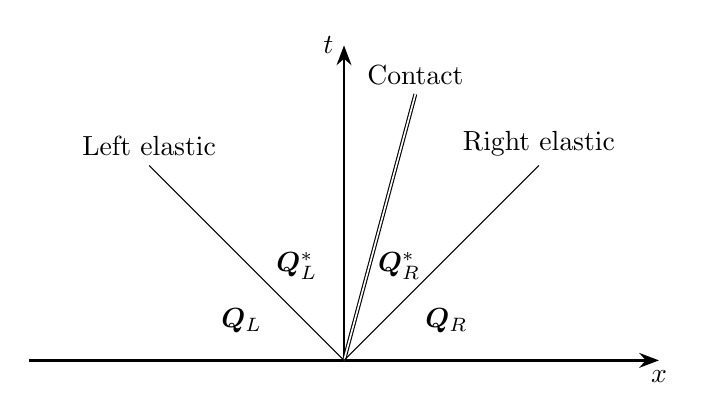
\begin{tikzpicture}
	\draw [line width =1pt,-{Stealth[length=2.5mm]}] (0,0) -- (4,0) node[below]{$x$};
	\draw [line width =1pt] (-4,0) -- (0,0);
	\draw [line width =1pt,-{Stealth[length=2.5mm]}] (0,0) -- (0,4) node[left]{$t$};
	%\draw (0,0)[dashed] node [below]{$O$} -- ([turn]-110:3.5) node [above]{Left plastic};
	\draw [double](0,0) -- ([turn]165:3.5)   node [above]{Contact};
	%\draw [dashed](0,0) -- ([turn]110:3.5)  node [above]{Right plastic};
	\draw  (0,0) -- ([turn]135:3.5) node [above]{Right elastic};
	\draw  (0,0) -- ([turn]-135:3.5) node [above]{Left elastic} ;
	\node at (-1.3,0.5) {$\bm{Q}_L$};
	%\node at (-1.2,0.8) {$\widetilde{\bm{Q}}_L$};
	\node at (-0.6,1.2) {$\bm{Q}_L^*$};
	\node at (0.7,1.2) {$\bm{Q}_R^*$};
	%\node at (1.2,0.8) {$\widetilde{\bm{Q}}_R$};
	\node at (1.3,0.5) {$\bm{Q}_R$};
	%\draw [-{Stealth[length=3mm]}] (0,0) -- (2,0);
\end{tikzpicture}
\caption{The  structures of HLLCEP method, case 1: without plastic wave.}
\label{fig:case1}
\end{figure}
According to the Rankine-Hugoniot conditions between left elastic wave,
\begin{equation} \label{eq:RH1}
	\bm{F}_L^* = \bm{F}_L+s_L (\bm{U}_L^*-\bm{U}_L),
\end{equation}
we can  get 
\begin{equation} \label{eq:rhoLstar}
  \rho_L^* u_L^*=\rho_L u_L+s_L(\rho_L^*-\rho_L),
\end{equation}
and
\begin{equation}\label{eq:sigma}
  \rho_L^* u_R^{*2}-\sigma^*_L=\rho_L u_L^2-\sigma_L+s_L(\rho_L^* u_L^*-\rho_L u_L).
\end{equation}
Using the relation of $u_L^* =u_R^* = s^*$ in Eq.(\ref{eq:contact}), the speed of contact wave can be evaluated as 
\begin{equation}
 \hat{s}^* = \frac{\sigma_L-\sigma_R+\rho_L u_L(s_L-u_L)-\rho_R u_R(s_R-u_R)}{\rho_L(s_L-u_L)-\rho_R(s_R-u_R)},
\end{equation}
the density is solved as
\begin{equation}\label{eq:rhoLs}
  \hat{\rho}_L^* = \frac{\rho_L(u_L-s_L)}{\hat{s}^*-s_L}.
\end{equation}
Samilar, we can get the density in the right 
\begin{equation}\label{eq:rhoLs}
  \hat{\rho}_R^* = \frac{\rho_R(u_R-s_R)}{\hat{s}^*-s_R}.
\end{equation}
where the speeds of left and right elastic waves are evaluted as 
	\begin{equation}\label{eq:sLR}
	  s_L = \text{min} (u_L-c_L, u_R-c_R), \hspace{0.3cm} s_R = \text{max}(u_L+c_L, u_R+c_R).
	\end{equation}
Based on the assumption above, as there is no plastic wave in, we can take the relation of Eq.(\ref{eq:rhosxx}), and the deviatoric stress is evaluated as 
\begin{equation}
  \hat{s}_{xxL}^*=-\frac{4}{3}\mu\text{ln}(\frac{\hat{\rho}_L^*}{\rho_L})+s_{xxL},\hspace{0.2cm}  \hat{s}_{xxR}^*=-\frac{4}{3}\mu\text{ln}(\frac{\hat{\rho}_R^*}{\rho_R})+s_{xxR}.
\end{equation}

If $|s_{xxL}|<\frac{2}{3}Y_0$ and $|\hat{s}_{xxL}^*| < \frac{2}{3}Y_0$, all the states in the left are not yielding. Or  $|s_{xxL}| \ge \frac{2}{3}Y_0$ and $|\hat{s}_{xxL}^*| \ge  \frac{2}{3}Y_0$, all the states in the left are yielding. The assumption  holds in the left. 
Meanwhile, if $|s_{xxR}|<\frac{2}{3}Y_0$ and $|\hat{s}_{xxR}^*| < \frac{2}{3}Y_0$, Or $|s_{xxR}| \ge \frac{2}{3}Y_0$ and $|\hat{s}_{xxR}^*| \ge  \frac{2}{3}Y_0$, the assumption holds in the right. Then the structures  truely are  the case in Fig.\ref{fig:case1}. 

Then 
\begin{align}
&  s^* = \hat{s}^*,\hspace{0.3cm} \rho^*_L = \hat{\rho}_L^*, \hspace{0.3cm} \rho_R^* = \hat{\rho}_R^*,\\
&  s_{xxL}^*  = \Upsilon(\hat{s}_{xxL}^*),\hspace{0.3cm} s_{xxR}^*  = \Upsilon(\hat{s}_{xxR}^*)
\end{align}
where,
\begin{equation}\label{eq:upsilon}
  \Upsilon(\omega) = \left\{ \begin{aligned}
	  &\omega, \hspace{0.3cm} \text{if} \hspace{0.3cm} |\omega| \le \frac{2}{3}Y_0,\\
	  &\frac{2}{3}Y_0,  \hspace{0.3cm} \text{if} \hspace{0.3cm} \omega > \frac{2}{3}Y_0,\\
	 &-\frac{2}{3}Y_0,  \hspace{0.3cm} \text{if} \hspace{0.3cm} \omega < -\frac{2}{3}Y_0.\\
 \end{aligned}\right.
 \end{equation}

 The Cauchy stresses are solved  by Eq.(\ref{eq:sigma}), 
\begin{equation*}
  \sigma_L^*=\sigma_R^*=\sigma_L -\rho_L (s_L-u_L)(s^*-u_L).
\end{equation*}
 Then we can get the pressure by $p =s_{xx}-\sigma$.
\begin{equation}
  p_L^* = s_{xxL}^* - \sigma_L^*, \hspace{0.3cm}   p_R^* = s_{xxR}^* - \sigma_R^*.
\end{equation}

 \subsubsection{Case 2:  with only the left plastic wave}\label{sec:case2}
 If $|s_{xxL}| \le \frac{2}{3}Y_0 \le  |\hat{s}_{xxL}^*|$, there exists a plastic wave in the left as showed in Fig.\ref{fig:case2}. We need to solve the state  of $\widetilde{\bm{Q}}_L$ at first. The HLLCEP is given as follows in this case,
 \begin{equation}\label{eq:HLLCEP2}
   \bm{U}^{\text{HLLCEP}}_{\text{Case2}}(x,t) = \left\{ \begin{aligned}
	   & \bm{U}_L, \hspace{0.3cm} \text{if} \hspace{0.3cm} \frac{x}{t}\le \widetilde{s}_L, \\
		&  \widetilde{\bm{U}}_L, \hspace{0.3cm} \text{if} \hspace{0.3cm} \widetilde{s}_L\le \frac{x}{t} \le  s_L, \\
		&\bm{U}_L^*, \hspace{0.3cm} \text{if} \hspace{0.3cm} s_L\le \frac{x}{t} \le s^*, \\
		& \bm{U}_R^*, \hspace{0.3cm} \text{if} \hspace{0.3cm} s^*\le \frac{x}{t} \le s_R,\\
		& \bm{U}_R, \hspace{0.3cm} \text{if} \hspace{0.3cm} \frac{x}{t}\ge s_R, \\
	  \end{aligned}
	\right.
  \end{equation}
  and the corresonding Eulerian and Lagrangian numerical flux are 
 \begin{equation}\label{eq:HLLCEP}
   \bm{F}^{\text{Euler}}_{\text{Case2}}(x,t) = \left\{ \begin{aligned}
	   & \bm{F}_L, \hspace{0.3cm} \text{if} \hspace{0.3cm} \frac{x}{t}\le \widetilde{s}_L, \\
		&  \widetilde{\bm{F}}_L, \hspace{0.3cm} \text{if} \hspace{0.3cm} \widetilde{s}_L\le \frac{x}{t} \le   s_L , \\
		&\bm{F}_L^*, \hspace{0.3cm} \text{if} \hspace{0.3cm} s_L\le \frac{x}{t} \le s^*, \\
		& \bm{F}_R^*, \hspace{0.3cm} \text{if} \hspace{0.3cm} s^*\le \frac{x}{t} \le s_R,\\
		& \bm{F}_R, \hspace{0.3cm} \text{if} \hspace{0.3cm} \frac{x}{t}\ge s_R, \\
	  \end{aligned}
	\right.
  \end{equation}
\begin{equation}
	\bm{F}^{\text{Lag}}_{\text{Case2}}(x,t) = \left\{ \begin{aligned}
		& \bm{f}_L^*, \hspace{0.3cm} \text{if} \hspace{0.3cm} s_*\ge \frac{x}{t},\\
		& \bm{f}_R^*, \hspace{0.3cm} \text{if} \hspace{0.3cm} s^*\le \frac{x}{t}.\\
	  \end{aligned}
	\right.
  \end{equation}


 \begin{figure}
   \centering 
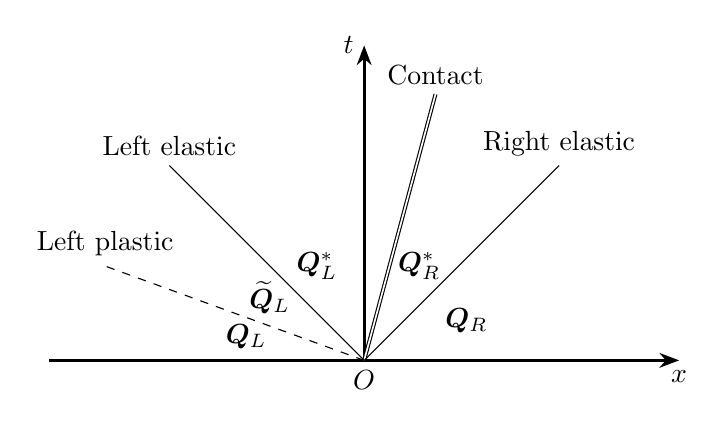
\begin{tikzpicture}
	\draw [line width =1pt,-{Stealth[length=2.5mm]}] (0,0) -- (4,0) node[below]{$x$};
	\draw [line width =1pt] (-4,0) -- (0,0);
	\draw [line width =1pt,-{Stealth[length=2.5mm]}] (0,0) -- (0,4) node[left]{$t$};
	\draw (0,0)[dashed] node [below]{$O$} -- ([turn]-110:3.5) node [above]{Left plastic};
	\draw [double](0,0) -- ([turn]165:3.5)   node [above]{Contact};
	%\draw [dashed](0,0) -- ([turn]110:3.5)  node [above]{Right plastic};
	\draw  (0,0) -- ([turn]135:3.5) node [above]{Right elastic};
	\draw  (0,0) -- ([turn]-135:3.5) node [above]{Left elastic} ;
	\node at (-1.5,0.3) {$\bm{Q}_L$};
	\node at (-1.2,0.8) {$\widetilde{\bm{Q}}_L$};
	\node at (-0.6,1.2) {$\bm{Q}_L^*$};
	\node at (0.7,1.2) {$\bm{Q}_R^*$};
	\node at (1.3,0.5) {$\bm{Q}_R$};
	%\draw [-{Stealth[length=3mm]}] (0,0) -- (2,0);
\end{tikzpicture}
\caption{The  structures of HLLCEP method, case 2: with only  the left plastic wave.}
\label{fig:case2}
\end{figure}
 Using the Rankine-Hugoniot relation of  the left  plastic wave,
  \begin{align}
	&\widetilde{\rho}_L(\widetilde{u}_L-\widetilde{s}_L) = \rho_L(u_L-\widetilde{s}_L), \label{eq:RHp1}\\
	&\widetilde{\rho}\widetilde{u}_L(\widetilde{u}_L-\widetilde{s}_L) = \rho_Lu_L(u_L-\widetilde{s}_L)+\widetilde{\sigma}_L-\sigma_L,  \label{eq:RHp2}\\
	&\widetilde{\rho}\widetilde{E}_L(\widetilde{u}_L-\widetilde{s}_L) = \rho_LE_L(u_L-\widetilde{s}_L)+\widetilde{\sigma}_L \widetilde{u}_L-\sigma_Lu_L, \label{eq:RHp3}
\end{align}
where yielding happened behind the plastic wave, so the deviatoric stress and density are taken as  
\begin{equation}
  \widetilde{s}_{xxL} =\left\{ \begin{aligned}
	  -\frac{2}{3}Y_0, \hspace{0.3cm} \text{if} \hspace{0.3cm} \rho_L^* > \rho_L,\\
	  \frac{2}{3}Y_0, \hspace{0.3cm} \text{if} \hspace{0.3cm} \rho_L^* < \rho_L,\\
	\end{aligned}\right.
  \end{equation}
  and
\begin{equation}   \widetilde{\rho}_{L} = \left\{ \begin{aligned}
	  & \rho_L \text{exp}\left(\frac{Y_0}{2\mu}+\frac{3 s_{xxL}}{4\mu}\right)  \hspace{0.5cm} \text{if} \hspace{0.3cm} \rho_L^* > \rho_L,\\ 
& \rho_L \text{exp}\left(-\frac{Y_0}{2\mu}+\frac{3 s_{xxL}}{4\mu}\right) 
\hspace{0.3cm} \text{if} \hspace{0.3cm} \rho_L^* < \rho_L.\\ 
  \end{aligned}\right.
 \end{equation}

 The unknowns are the wave speed $\widetilde{s}_L$,  the velocity  $\widetilde{u}_L$, the pressure $\widetilde{p}_L$ and the specific internal energy $\widetilde{E}_L$. In the following, we will give the derivations of   

 From Eq.(\ref{eq:RHp1}) we can get the wave speed
  \begin{equation}
	\widetilde{s}_L = \frac{\widetilde{\rho}_L \widetilde{u}_L-\rho_Lu_L}{\widetilde{\rho}_L-\rho_L},
  \end{equation}
and the relation
\begin{equation}\label{eq:u1_s}
  u_L-\widetilde{s}_L = \frac{(u_L-\widetilde{u}_L)\widetilde{\rho}_L}{\widetilde{\rho}_L-\rho_L}. 
\end{equation}
Substituting Eq.(\ref{eq:RHp1}) into Eq.(\ref{eq:RHp2}), we have 
\begin{equation}\label{eq:rho1}
  \rho_L(\widetilde{u}_L - u_L)(u_L-\widetilde{s}_L) = \widetilde{\sigma}_L -\sigma_L,
\end{equation}
then substituting Eq.(\ref{eq:u1_s}) into it, we can get the following relation
\begin{equation}\label{eq:tu_2}
  -t(\widetilde{u}_L-u_L)^2 = \widetilde{\sigma}_L-\sigma_L,
\end{equation}
where
\begin{equation}
t=\frac{\rho_L \widetilde{\rho}_L}{\widetilde{\rho}_L-\rho_L}.
\end{equation}
Similar to Eq.(\ref{eq:rho1}), Eq.(\ref{eq:RHp2}) can be changed into 
\begin{equation}
  t(u_L-\widetilde{u}_L)(\widetilde{E}_L-E_L) =\widetilde{\sigma}_L\widetilde{u}_L-\sigma_Lu_L,
\end{equation}
and we also know that $E = e+\frac{1}{2}u^2$, then we have 
\begin{equation}\label{eq:e21}
  \widetilde{e}_L-e_L= -\frac{\sigma_L+\widetilde{\sigma}_L}{2t}.
\end{equation}
The EOS (\ref{eq:mie}) can be written as
\begin{equation} \label{eq:eos1}
  e=c_0 p-c_1f(\rho/\rho_0),
\end{equation}
where $c_0=\frac{1}{\rho_0\Gamma_0}$ and $c_1=\frac{a_0^2}{\Gamma_0}$.  

Substituting (\ref{eq:eos1}) and $\sigma=-p +s_{xx}$ into (\ref{eq:e21}), we can get the pressure behind the plastic wave as
\begin{equation}
  \widetilde{p}_L= \frac{2t(c_1f(\widetilde{\rho}_L)+e_L)-(\sigma_L+\widetilde{s}_{xxL})}{2tc_0-1},
\end{equation}
and the Cauchy stress is solved by $\widetilde{\sigma}_L = -\widetilde{p}_L+\widetilde{s}_{xxL}$. Using Eq.(\ref{eq:tu_2}) we can get
\begin{equation}
  (\widetilde{u}_L-u_L)^2 = \frac{\sigma_L-\widetilde{\sigma}_L}{t},
\end{equation}
then the velocity is solved,
\begin{equation}
  \widetilde{\bm{u}}_L= \left\{
  \begin{aligned}
	u_L+\sqrt{\frac{\sigma_L-\widetilde{\sigma}_L}{t}} \hspace{0.2cm} \text{if} \hspace{0.2cm} \rho_R^* >\rho_R,\\
	u_L-\sqrt{\frac{\sigma_L-\widetilde{\sigma}_L}{t}} \hspace{0.2cm} \text{if} \hspace{0.2cm} \rho_R^* <\rho_R.\\
\end{aligned} \right.
\end{equation}

After solve the state of $\widetilde{\bm{Q}}_L$,  using a samilar process with Section \ref{sec:case1}, the states of $\bm{Q}_L^*$ and $\bm{Q}_R^*$ can be solved out.

Solving the contace wave speed,
\begin{equation}
  s^* = \frac{\widetilde{\sigma}_L-\sigma_R+\widetilde{\rho}_L \widetilde{u}_L(s_L-\widetilde{u}_L)-\rho_R u_R(s_R-u_R)}{\widetilde{\rho}_L(s_L-\widetilde{u}_L)-\rho_R(s_R-u_R)},
\end{equation}

Solving the densities,
\begin{equation}
  \rho_L^* = \frac{\widetilde{\rho}_L(\widetilde{u}_L-s_L)}{s^*-s_L}, \hspace{0.3cm}  \rho_R^* = \frac{\rho_R(u_R-s_R)}{s^*-s_R},
\end{equation}
where  the left and right  elastic wave speeds are evaluted as 
	\begin{equation}
	  s_L = \text{min} (\widetilde{u}_L-\widetilde{c}_L, u_R-c_R), \hspace{0.3cm} s_R = \text{max}(\widetilde{u}_L+\widetilde{c}_L, u_R+c_R).
	\end{equation}

The deviatoric stresses are evaluated as 
\begin{equation}
  \overline{s}_{xxL}^*=-\frac{4}{3}\mu\text{ln}(\frac{\rho_L^*}{\rho_L})+s_{xxL},\hspace{0.2cm}  \overline{s}_{xxR}^*=-\frac{4}{3}\mu\text{ln}(\frac{\rho_R^*}{\rho_R})+s_{xxR},
\end{equation}
then using von Mises' yielding condition 
\begin{equation}
  s_{xxL}^* = \Upsilon(\overline{s}_{xxL}^*), \hspace{0.3cm}  s_{xxR}^* = \Upsilon(\overline{s}_{xxR}^*). 
\end{equation}
The Cauchy stresses are given as
\begin{equation}
  \sigma_L^*=\sigma_R^*=\widetilde{\sigma}_L -\widetilde{\rho}_L (s_L-\widetilde{u}_L)(s^*-\widetilde{u}_L),
\end{equation}
and the pressures are 
\begin{equation}
  p_L^* = s_{xxL}^* - \sigma_L^*, \hspace{0.3cm}   p_R^* = s_{xxR}^* - \sigma_R^*.
\end{equation}

\subsubsection {Case 3: with only the  right plastic wave}\label{sec:case3}
If  $|s_{xxR}| \le \frac{2}{3}Y_0 \le  |\hat{s}_{xxR}^*|$, there exists a plastic wave in the right as showed in Fig.\ref{fig:case3}. We need to solve the state  of $\widetilde{\bm{Q}}_R$ at first. The HLLCEP is given in this case as,

 \begin{equation}\label{eq:HLLCEP3}
   \bm{U}^{\text{HLLCEP}}_{\text{Case3}}(x,t) = \left\{ \begin{aligned}
		& \bm{U}_L, \hspace{0.3cm} \text{if} \hspace{0.3cm} \frac{x}{t}\le s_L, \\
		& \bm{U}_L^*, \hspace{0.3cm} \text{if} \hspace{0.3cm} s_L \le \frac{x}{t} \le s^*, \\
		& \bm{U}_R^*, \hspace{0.3cm} \text{if} \hspace{0.3cm} s^*\le \frac{x}{t} \le s_R, \\
		& \widetilde{\bm{U}}_R, \hspace{0.3cm} \text{if} \hspace{0.3cm} s_R \le \frac{x}{t} \le \widetilde{s}_R,\\
		& \bm{U}_R, \hspace{0.3cm} \text{if} \hspace{0.3cm} \frac{x}{t}\ge \widetilde{s}_R, \\
	  \end{aligned}
	\right.
  \end{equation}

  and the corresonding Eulerian and Lagrangian numerical flux are 
 \begin{equation}\label{eq:HLLCEP3}
   \bm{F}^{\text{Euler}}_{\text{Case3}}(x,t) = \left\{ \begin{aligned}
		& \bm{F}_L, \hspace{0.3cm} \text{if} \hspace{0.3cm} \frac{x}{t}\le s_L, \\
		& \bm{F}_L^*, \hspace{0.3cm} \text{if} \hspace{0.3cm} s_L\le \frac{x}{t} \le s^*, \\
		& \bm{F}_R^*, \hspace{0.3cm} \text{if} \hspace{0.3cm} s^*\le \frac{x}{t} \le s_R, \\
		&  \widetilde{\bm{F}}_R, \hspace{0.3cm} \text{if} \hspace{0.3cm} s_R\le \frac{x}{t} \le \widetilde{s}_R,\\
		& \bm{F}_R, \hspace{0.3cm} \text{if} \hspace{0.3cm} \frac{x}{t}\ge \widetilde{s}_R, \\
	  \end{aligned}
	\right.
  \end{equation}
\begin{equation}
	\bm{F}^{\text{Lag}}_{\text{Case3}}(x,t) = \left\{ \begin{aligned}
		& \bm{f}_L^*, \hspace{0.3cm} \text{if} \hspace{0.3cm} s_*\ge \frac{x}{t},\\
		& \bm{f}_R^*, \hspace{0.3cm} \text{if} \hspace{0.3cm} s^*\le \frac{x}{t}.\\
	  \end{aligned}
	\right.
  \end{equation}

The deviatoric stress, density and pressure are given as 
\begin{equation}
  \widetilde{s}_{xxR} =\left\{ \begin{aligned}
	  -\frac{2}{3}Y_0, \hspace{0.3cm} \text{if} \hspace{0.3cm} \rho_R^* > \rho_R,\\
	  \frac{2}{3}Y_0, \hspace{0.3cm} \text{if} \hspace{0.3cm} \rho_R^* < \rho_R,\\
	\end{aligned}\right.
	\hspace{0.2cm} \widetilde{\rho}_{R} = \left\{ \begin{aligned}
	  & \rho_R \text{exp}\left(\frac{Y_0}{2\mu}+\frac{3 s_{xxR}}{4\mu}\right)  \hspace{0.5cm} \text{if} \hspace{0.3cm} \rho_R^* > \rho_R,\\ 
& \rho_R \text{exp}\left(-\frac{Y_0}{2\mu}+\frac{3 s_{xxR}}{4\mu}\right) 
\hspace{0.3cm} \text{if} \hspace{0.3cm} \rho_R^* < \rho_R,\\ 
  \end{aligned}\right.
 \end{equation}
\begin{equation}
  \widetilde{p}_R= \frac{2t(c_1f(\widetilde{\rho}_R)+e_R)-(\sigma_R+\widetilde{s}_{xxR})}{2tc_0-1}, \hspace{0.3cm} 
t=\frac{\rho_R \widetilde{\rho}_R}{\widetilde{\rho}_R-\rho_R},
\end{equation}
where $c_0 =\frac{1}{\rho_0 \Gamma_0}$ and $c_1 = \frac{a_0^2}{\Gamma_0}$.
The Cauchy stress and velocity are
\begin{equation}
\widetilde{\sigma}_R = -\widetilde{p}_R+\widetilde{s}_{xxR},
\end{equation}
\begin{equation}
  \widetilde{u}_R= \left\{
  \begin{aligned}
	u_R+\sqrt{\frac{\sigma_R-\widetilde{\sigma}_R}{t}} \hspace{0.2cm} \text{if} \hspace{0.2cm} \rho_R^* >\rho_R,\\
	u_R-\sqrt{\frac{\sigma_R-\widetilde{\sigma}_R}{t}} \hspace{0.2cm} \text{if} \hspace{0.2cm} \rho_R^* <\rho_R.\\
\end{aligned} \right.
\end{equation}

\begin{figure}
  \centering
 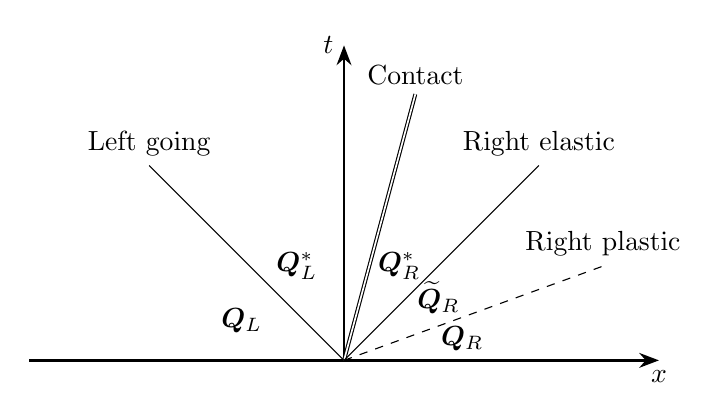
\begin{tikzpicture}
	\draw [line width =1pt,-{Stealth[length=2.5mm]}] (0,0) -- (4,0) node[below]{$x$};
	\draw [line width =1pt] (-4,0) -- (0,0);
	\draw [line width =1pt,-{Stealth[length=2.5mm]}] (0,0) -- (0,4) node[left]{$t$};
	%\draw (0,0)[dashed] node [below]{$O$} -- ([turn]-110:3.5) node [above]{Left plastic};
	\draw [double](0,0) -- ([turn]165:3.5)   node [above]{Contact};
	\draw [dashed](0,0) -- ([turn]110:3.5)  node [above]{Right plastic};
	\draw  (0,0) -- ([turn]135:3.5) node [above]{Right elastic};
	\draw  (0,0) -- ([turn]-135:3.5) node [above]{Left going} ;
	\node at (-1.3,0.5) {$\bm{Q}_L$};
	%\node at (-1.2,0.8) {$\widetilde{\bm{Q}}_L$};
	\node at (-0.6,1.2) {$\bm{Q}_L^*$};
	\node at (0.7,1.2) {$\bm{Q}_R^*$};
	\node at (1.2,0.8) {$\widetilde{\bm{Q}}_R$};
	\node at (1.5,0.28) {$\bm{Q}_R$};
	%\draw [-{Stealth[length=3mm]}] (0,0) -- (2,0);
\end{tikzpicture}
\caption{The  structures of HLLCEP method, case 3: with only  the right  plastic wave.}
\label{fig:case3}
\end{figure}

After solving the state of $\widetilde{\bm{Q}}_R$, we can solve the states of $\bm{Q}_L^*$ and  $\bm{Q}_R^*$.

The contact wave speed is 
\begin{equation}
  s^* = \frac{\sigma_L-\widetilde{\sigma}_R+\rho_L u_L(s_L-u_L)-\widetilde{\rho}_R \widetilde{u}_R(s_R-\widetilde{u}_R)}{\rho_L(s_L-u_L)-\widetilde{\rho}_R(s_R-\widetilde{u}_R)}.
\end{equation}
The densities are
\begin{equation}\label{eq:rhoLs}
  \rho_L^* = \frac{\rho_L(u_L-s_L)}{s^*-s_L}, \hspace{0.3cm}  \rho_R^* = \frac{\widetilde{\rho}_R(\widetilde{u}_R-s_R)}{s^*-s_R},
\end{equation}
where the left and right elastic wave speeds are
	\begin{equation}
	  s_L = \text{min} (u_L-c_L, \widetilde{u}_R-\widetilde{c}_R), \hspace{0.3cm} s_R = \text{max}(u_L+c_L, \widetilde{u}_R+\widetilde{c}_R).
	\end{equation}
	The deviatoric stresses are 
\begin{equation}
  \overline{s}_{xxL}^*=-\frac{4}{3}\mu\text{ln}(\frac{\rho_L^*}{\rho_L})+s_{xxL},\hspace{0.2cm}  \overline{s}_{xxR}^*=-\frac{4}{3}\mu\text{ln}(\frac{\rho_R^*}{\rho_R})+s_{xxR},
\end{equation}
\begin{equation}
  s_{xxL}^* = \Upsilon(\overline{s}_{xxL}^*), \hspace{0.3cm}  s_{xxR}^* = \Upsilon(\overline{s}_{xxR}^*). 
\end{equation}
The Cauchy stresses are
\begin{equation}
  \sigma_L^*=\sigma_R^*=\sigma_L -\rho_L (s_L-u_L)(s^*-u_L),
\end{equation}
and the pressures are 
\begin{equation}
  p_L^* = s_{xxL}^* - \sigma_L^*, \hspace{0.3cm}   p_R^* = s_{xxR}^* - \sigma_R^*.
\end{equation}



\subsubsection{Case4: with both the left and right plastic waves}

If $|s_{xxL}| \le \frac{2}{3}Y_0 \le  |\hat{s}_{xxL}^*|$ and  $|s_{xxR}| \le \frac{2}{3}Y_0 \le  |\hat{s}_{xxR}^*|$. Both  the left side  and right side exist plastic waves, as showed in Fig.\ref{fig:case4}. The HLLCEP Riemann solver is given as
 \begin{equation}
   \bm{U}^{\text{HLLCEP}}_{\text{Case4}}(x,t) = \left\{ \begin{aligned}
		& \bm{U}_L, \hspace{0.3cm} \text{if} \hspace{0.3cm} \frac{x}{t}\le s_L, \\
		& \bm{U}_L^*, \hspace{0.3cm} \text{if} \hspace{0.3cm} s_L\le \frac{x}{t} \le \widetilde{s}_L, \\
		& \widetilde{\bm{U}}_L, \hspace{0.3cm} \text{if} \hspace{0.3cm} \widetilde{s}_L\le \frac{x}{t} \le s^*, \\
		& \widetilde{\bm{U}}_R, \hspace{0.3cm} \text{if} \hspace{0.3cm} s^*\le \frac{x}{t} \le \widetilde{s}_R, \\
		& \bm{U}_R^*, \hspace{0.3cm} \text{if} \hspace{0.3cm} \widetilde{s}_R\le \frac{x}{t} \le s_R,\\
		& \bm{U}_R, \hspace{0.3cm} \text{if} \hspace{0.3cm} \frac{x}{t}\ge s_R, \\
	  \end{aligned}
	\right.
  \end{equation}
  and the corresonding Eulerian and Lagrangian numerical flux are 
 \begin{equation}\label{eq:HLLCEP}
   \bm{F}^{\text{Euler}}_{\text{Case4}}(x,t) = \left\{ \begin{aligned}
		& \bm{F}_L, \hspace{0.3cm} \text{if} \hspace{0.3cm} \frac{x}{t}\le s_L, \\
		& \bm{F}_L^*, \hspace{0.3cm} \text{if} \hspace{0.3cm} \widetilde{s}_L\le \frac{x}{t} \le s_L, \\
		& \widetilde{\bm{F}}_L, \hspace{0.3cm} \text{if} \hspace{0.3cm} s_L\le \frac{x}{t} \le s^*, \\
		& \widetilde{\bm{F}}_R, \hspace{0.3cm} \text{if} \hspace{0.3cm} s^*\le \frac{x}{t} \le s_R, \\
		& \bm{F}_R^*, \hspace{0.3cm} \text{if} \hspace{0.3cm} s_R\le \frac{x}{t} \le\widetilde{ s}_R,\\
		& \bm{F}_R, \hspace{0.3cm} \text{if} \hspace{0.3cm} \frac{x}{t}\ge s_R, \\
	  \end{aligned}
	\right.
  \end{equation}

\begin{equation}
\bm{F}^{\text{Lag}}_{\text{Case4}}(x,t) = \left\{ \begin{aligned}
		& \widetilde{\bm{f}}_L, \hspace{0.3cm} \text{if} \hspace{0.3cm} s_*\ge \frac{x}{t},\\
		& \widetilde{\bm{f}}_R, \hspace{0.3cm} \text{if} \hspace{0.3cm} s^*\le \frac{x}{t}.\\
	  \end{aligned}
	\right.
  \end{equation}

\begin{figure}
  \centering
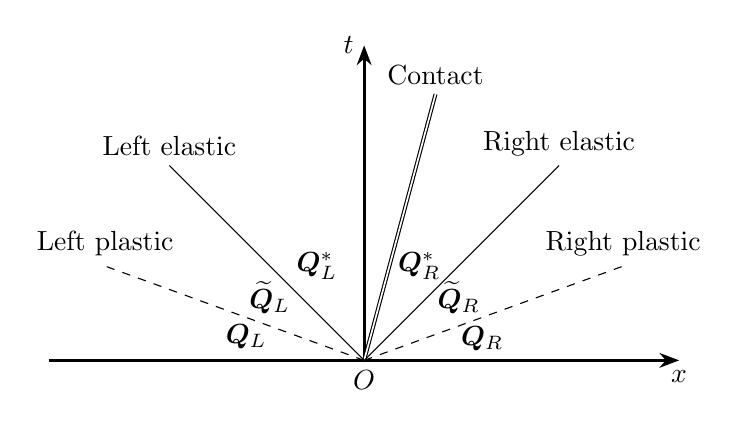
\begin{tikzpicture}
	\draw [line width =1pt,-{Stealth[length=2.5mm]}] (0,0) -- (4,0) node[below]{$x$};
	\draw [line width =1pt] (-4,0) -- (0,0);
	\draw [line width =1pt,-{Stealth[length=2.5mm]}] (0,0) -- (0,4) node[left]{$t$};
	\draw (0,0)[dashed] node [below]{$O$} -- ([turn]-110:3.5) node [above]{Left plastic};
	\draw [double](0,0) -- ([turn]165:3.5)   node [above]{Contact};
	\draw [dashed](0,0) -- ([turn]110:3.5)  node [above]{Right plastic};
	\draw  (0,0) -- ([turn]135:3.5) node [above]{Right elastic};
	\draw  (0,0) -- ([turn]-135:3.5) node [above]{Left elastic} ;
	\node at (-1.5,0.3) {$\bm{Q}_L$};
	\node at (-1.2,0.8) {$\widetilde{\bm{Q}}_L$};
	\node at (-0.6,1.2) {$\bm{Q}_L^*$};
	\node at (0.7,1.2) {$\bm{Q}_R^*$};
	\node at (1.2,0.8) {$\widetilde{\bm{Q}}_R$};
	\node at (1.5,0.28) {$\bm{Q}_R$};
	%\draw [-{Stealth[length=3mm]}] (0,0) -- (2,0);
\end{tikzpicture}
\caption{The  structures of HLLCEP method, case 4: with both left and right plastic waves.}
\label{fig:case4}
\end{figure}

The states of $\widetilde{\bm{Q}}_L$ and   $\widetilde{\bm{Q}}_R$ can be solved by the same process with Section \ref{sec:case2} and Section \ref{sec:case3}. Then the states of $\bm{Q}^*_L$ and $\bm{Q}^*_R$ are given as following.

The speed of waves are evaluted as
\begin{equation}
  s_L = \text{min} (\widetilde{u}_L-\widetilde{c}_L, \widetilde{u}_R-\widetilde{c}_R), \hspace{0.3cm} s_R = \text{max}(\widetilde{u}_L+\widetilde{c}_L, \widetilde{u}_R+\widetilde{c}_R),
	\end{equation}
	\begin{equation}
	  s^* = \frac{\widetilde{\sigma}_L-\widetilde{\sigma}_R+\widetilde{\rho}_L \widetilde{u}_L(s_L-\widetilde{u}_L)-\widetilde{\rho}_R \widetilde{u}_R(s_R-\widetilde{u}_R)}{\widetilde{\rho}_L(s_L-\widetilde{u}_L)-\widetilde{\rho}_R(s_R-\widetilde{u}_R)}.
\end{equation}
Then we can get the density using Eq.(\ref{eq:rhoLs}),
\begin{equation}
  \rho_L^* = \frac{\widetilde{\rho}_L(\widetilde{u}_L-s_L)}{s^*-s_L}, \hspace{0.3cm}  \rho_R^* = \frac{\widetilde{\rho}_R(\widetilde{u}_R-s_R)}{s^*-s_R},
\end{equation}
and the deviatoric stress using Eq.(\ref{eq:sxxrho}),
  \begin{align}
  \overline{s}_{xxL}^* =  -\frac{4}{3}\mu \text{ln}\left( \frac{\rho_L^*}{\rho_L}  \right)+s_{xxL},\\
  \overline{s}_{xxR}^* =  -\frac{4}{3}\mu \text{ln}\left( \frac{\rho_R^*}{\rho_R}  \right)+s_{xxR},\\
\end{align}
then using  the von Mises' yielding condition,
\begin{equation}
  s_{xxL}^* = \Upsilon(\overline{s}_{xxL}^*) , \hspace{0.3cm}  s_{xxR}^* = \Upsilon(\overline{s}_{xxR}^*).
\end{equation}
The Cauchy stresses  are solved as 
\begin{equation}
  \sigma_L^*=\sigma_R^*=\widetilde{\sigma}_L -\widetilde{\rho_L} (s_L-\widetilde{u}_L)(s^*-\widetilde{u}_L).
\end{equation}
So we can get the pressure by $p =s_{xx}-\sigma$,
\begin{equation}
  p_L^* = s_{xxL}^* - \sigma_L^*, \hspace{0.3cm}   p_R^* = s_{xxR}^* - \sigma_R^*.
\end{equation}


\subsection{Summary of HLLCEP}
Here, we present all the procedures of HLLCEP in  a more simple way.

Step 1  Evaluate  $\hat{s}^*$
\begin{equation*}
  \hat{s}^* = \frac{\sigma_L-\sigma_R+\rho_L u_L(s_L-u_L)-\rho_R u_R(s_R-u_R)}{\rho_L(s_L-u_L)-\rho_R(s_R-u_R)}.
\end{equation*}

Step 2  Evaluate  $\hat{\rho}_L^*$ and $\hat{\rho}_R^*$
\begin{equation*}
  \hat{\rho}_L^* = \frac{\rho_L(u_L-s_L)}{s^*-s_L}, \hspace{0.3cm}  \hat{\rho}_R^* = \frac{\rho_R(u_R-s_R)}{s^*-s_R}.
\end{equation*}

Step 3  Evaluate  the deviatoric stress
\begin{equation*}
  \hat{s}_{xxL}^*=-\frac{4}{3}\mu\text{ln}(\frac{\hat{\rho}_L^*}{\rho_L})+s_{xxL},\hspace{0.2cm}  \hat{s}_{xxR}^*=-\frac{4}{3}\mu\text{ln}(\frac{\hat{\rho}_R^*}{\rho_R})+s_{xxR}.
\end{equation*}

Step 4 Solve the state behind the left  plastic wave

\vspace{0.3cm} \hspace{0.4cm}  If $|s_{xxL}| < \frac{2}{3}Y_0 \le |\hat{s}_{xxL}^*| $, left plastic wave exists, the deviatoric stress, density and pressure  are given as
\begin{equation*}
  \widetilde{s}_{xxL} =\left\{ \begin{aligned}
	  -\frac{2}{3}Y_0, \hspace{0.3cm} \text{if} \hspace{0.3cm} \rho_L^* > \rho_L,\\
	  \frac{2}{3}Y_0, \hspace{0.3cm} \text{if} \hspace{0.3cm} \rho_L^* < \rho_L,\\
	\end{aligned}\right.
	\hspace{0.2cm} \widetilde{\rho}_{L} = \left\{ \begin{aligned}
	  & \rho_L \text{exp}\left(\frac{Y_0}{2\mu}+\frac{3 s_{xxL}}{4\mu}\right)  \hspace{0.5cm} \text{if} \hspace{0.3cm} \rho_L^* > \rho_L,\\ 
& \rho_L \text{exp}\left(-\frac{Y_0}{2\mu}+\frac{3 s_{xxL}}{4\mu}\right) 
\hspace{0.3cm} \text{if} \hspace{0.3cm} \rho_L^* < \rho_L,\\ 
  \end{aligned}\right.
 \end{equation*}
\begin{equation*}
  \widetilde{p}_L= \frac{2t(c_1f(\widetilde{\rho}_L)+e_L)-(\sigma_L+\widetilde{s}_{xxL})}{2tc_0-1}, \hspace{0.3cm} 
t=\frac{\rho_L \widetilde{\rho}_L}{\widetilde{\rho}_L-\rho_L},
\end{equation*}
and the Cauchy stress and velocity are
\begin{equation*}
\widetilde{\sigma}_L = -\widetilde{p}_L+\widetilde{s}_{xxL},
\end{equation*}
\begin{equation*}
  \widetilde{u}_L= \left\{
  \begin{aligned}
	u_L-\sqrt{\frac{\sigma_L-\widetilde{\sigma}_L}{t}} \hspace{0.2cm} \text{if} \hspace{0.2cm} \rho_L^* >\rho_L,\\
	u_L+\sqrt{\frac{\sigma_L-\widetilde{\sigma}_L}{t}} \hspace{0.2cm} \text{if} \hspace{0.2cm} \rho_L^* <\rho_L.\\
\end{aligned} \right.
\end{equation*}
If left plactic wave does not exist,
\begin{equation*}
  \widetilde{\bm{Q}}_L = \bm{Q}_L.
\end{equation*}

Step 5 Solve the state behind the right plastic wave

\vspace{0.3cm} \hspace{0.4cm}  If $|s_{xxR}| < \frac{2}{3}Y_0 \le |\hat{s}_{xxR}^*| $, right plastic wave exists, the deviatoric stress, density and pressure  are given as
\begin{equation*}
  \widetilde{s}_{xxR} =\left\{ \begin{aligned}
	  -\frac{2}{3}Y_0, \hspace{0.3cm} \text{if} \hspace{0.3cm} \rho_R^* > \rho_R,\\
	  \frac{2}{3}Y_0, \hspace{0.3cm} \text{if} \hspace{0.3cm} \rho_R^* < \rho_R,\\
	\end{aligned}\right.
	\hspace{0.2cm} \widetilde{\rho}_{R} = \left\{ \begin{aligned}
	  & \rho_R \text{exp}\left(\frac{Y_0}{2\mu}+\frac{3 s_{xxR}}{4\mu}\right)  \hspace{0.5cm} \text{if} \hspace{0.3cm} \rho_R^* > \rho_R,\\ 
& \rho_R \text{exp}\left(-\frac{Y_0}{2\mu}+\frac{3 s_{xxR}}{4\mu}\right) 
\hspace{0.3cm} \text{if} \hspace{0.3cm} \rho_R^* < \rho_R,\\ 
  \end{aligned}\right.
 \end{equation*}
\begin{equation*}
  \widetilde{p}_R= \frac{2t(c_1f(\widetilde{\rho}_R)+e_R)-(\sigma_R+\widetilde{s}_{xxR})}{2tc_0-1}, \hspace{0.3cm} 
t=\frac{\rho_R \widetilde{\rho}_R}{\widetilde{\rho}_R-\rho_R},
\end{equation*}
and the Cauchy stress and velocity are
\begin{equation*}
\widetilde{\sigma}_R = -\widetilde{p}_R+\widetilde{s}_{xxR},
\end{equation*}
\begin{equation*}
  \widetilde{u}_R= \left\{
  \begin{aligned}
	u_R+\sqrt{\frac{\sigma_R-\widetilde{\sigma}_R}{t}} \hspace{0.2cm} \text{if} \hspace{0.2cm} \rho_R^* >\rho_R,\\
	u_R-\sqrt{\frac{\sigma_R-\widetilde{\sigma}_R}{t}} \hspace{0.2cm} \text{if} \hspace{0.2cm} \rho_R^* <\rho_R.\\
\end{aligned} \right.
\end{equation*}
If right  plactic wave does not exist,
\begin{equation*}
  \widetilde{\bm{Q}}_R = \bm{Q}_R.
\end{equation*}

Step 6  Solve the wave speeds,
\begin{equation*}
  s_L = \text{min} (\widetilde{u}_L-\widetilde{c}_L, \widetilde{u}_R-\widetilde{c}_R), \hspace{0.3cm} s_R = \text{max}(\widetilde{u}_L+\widetilde{c}_L, \widetilde{u}_R+\widetilde{c}_R),
	\end{equation*}
	\begin{equation*}
	  s^* = \frac{\widetilde{\sigma}_L-\widetilde{\sigma}_R+\widetilde{\rho}_L \widetilde{u}_L(s_L-\widetilde{u}_L)-\widetilde{\rho}_R \widetilde{u}_R(s_R-\widetilde{u}_R)}{\widetilde{\rho}_L(s_L-\widetilde{u}_L)-\widetilde{\rho}_R(s_R-\widetilde{u}_R)}.
\end{equation*}

Step 7  Solve the densities,
\begin{equation*}
  \rho_L^* = \frac{\widetilde{\rho}_L(\widetilde{u}_L-s_L)}{s^*-s_L}, \hspace{0.3cm}  \rho_R^* = \frac{\widetilde{\rho}_R(\widetilde{u}_R-s_R)}{s^*-s_R},
\end{equation*}

Step 8 Solve the deviatoric stresses,
 \begin{align*}
  \hat{s}_{xxL}^* =  -\frac{4}{3}\mu \text{ln}\left( \frac{\rho_L^*}{\rho_L}  \right)+s_{xxL},\\
  \hat{s}_{xxR}^* =  -\frac{4}{3}\mu \text{ln}\left( \frac{\rho_R^*}{\rho_R}  \right)+s_{xxR},\\
\end{align*}
then using  the von Mises' yielding condition,
\begin{equation*}
  s_{xxL}^* = \Upsilon(\hat{s}_{xxL}^*) , \hspace{0.3cm}  s_{xxR}^* = \Upsilon(\hat{s}_{xxR}^*).
\end{equation*}

Step 9  Solving the Cauchy stresses,
\begin{equation*}
  \sigma_L^*=\sigma_R^*=\widetilde{\sigma}_L -\widetilde{\rho_L} (s_L-\widetilde{u}_L)(s^*-\widetilde{u}_L).
\end{equation*}
 Then we can get the pressure by $p =s_{xx}-\sigma$.

 \section{ A High-order cell-centered Lagrangian scheme for 1D  conservative hydrodynamic equations with Wilkins' model}
Here, we consider the following governing equations with Wilkins' model,

\begin{equation}\label{eq:gveq}
   \left\{ \begin{aligned}
	   & \partial _t \rho +\partial_x(\rho u)=0,\\
	   & \partial _t (\rho u)+\partial_x(\rho u^2 + p -s_{xx})=0,\\
	   &\partial _t (\rho E)+\partial_x([\rho E + p -s_{xx}]u)=0,\\
	   &\partial _t s_{xx}+u\partial_xs_{xx}-\frac{4}{3}\partial_x u=0,\\
	   \end{aligned}\right.
\end{equation}
where $Q = (\rho, \rho u, \rho E, s_{xx})^T$.  For a Lagrangian scheme, the governing equations also include the equation for moving the coordinates at the vertex of the mesh,
\begin{equation}\label{eq:dxt}
  \frac{dx(t)}{dt} = u(x,t).
\end{equation}

The spatial domain is discretized into $N$ cells $I_i = [x_{i-1/2}, x_{i+1/2}]$ of space sizes $\Delta x_i = x_{i+1/2} - x_{i-1/2}$ for $i = 1,2,\cdots,N$. For a given cell $I_i$, the cell center is denoted by $x_i$. The velocity $u_{i+1/2}$ is defined at the vertex of the mesh. The  value of the cell average for the cell $I_i$ is defined by
\begin{equation}
  \overline{\bm{Q}}_i = \frac{1}{\Delta x_i} \int_{I_i} \bm{Q} dx.
\end{equation}
\subsection{Spatial discretization}
The  semi-discrete finite volume scheme of the conservative equations (\ref{eq:gveq}) in the cell $I_i$ is written as
\begin{equation}\label{eq:sem}
  \frac{d(\overline{\bm{U}}_i\Delta x_i)}{dt} = -(\bm{F}_{i+\frac{1}{2}} - \bm{F}_{i-\frac{1}{2}}),
\end{equation}
where 
\begin{equation}
  \bm{F}_{i+\frac{1}{2}} = \bm{\Phi} (\bm{Q}_{L,i+\frac{1}{2}}, \bm{Q}_{R,i+\frac{1}{2}})  = \left[ 
	\begin{array}{l}
	  0\\
	  p_{i+\frac{1}{2}} - (s_{xx})_{i+\frac{1}{2}}\\
	  (p_{i+\frac{1}{2}} - (s_{xx})_{i+\frac{1}{2}})u_{i+\frac{1}{2}}\\
	\end{array}
  \right],
\end{equation}
$\bm{Q}_{L,i+\frac{1}{2}}$ and $\bm{Q}_{R,i+\frac{1}{2}}$ represent the left and right values of $\bm{Q}$ at the cell's boundary $x_{i+\frac{1}{2}}$, and  $p_{i+\frac{1}{2}}$, $(s_{xx})_{i+\frac{1}{2}}$ and $u_{i+\frac{1}{2}}$ denote the Godunov values at $x_{i+\frac{1}{2}}$, respectively. 

The Godunov values  $\bm{Q}_{i+\frac{1}{2}}$  can be solved  by the Riemiann problem  (\ref{eq:1d}) at $x_{i+\frac{1}{2}}$, 
\begin{equation}
  \bm{Q}_{i+\frac{1}{2}} = \left\{ \begin{aligned}
	\bm{Q}_L^*, \hspace{0.3cm} \text{if} \hspace{0.3cm} \frac{dx}{dt} \le  s^*,\\
	\bm{Q}_R^*, \hspace{0.3cm} \text{if} \hspace{0.3cm} \frac{dx}{dt} > s^*,\\
  \end{aligned} \right.
\end{equation}
where $\bm{Q}_L^*$, $\bm{Q}_R^*$ and $s^*$ are evaluated by the HLLCEP in section \ref{sec:HLLCEP}.

Before this, we must give the left  and right initial value ($\bm{Q}_{L,i+\frac{1}{2}}$ and $\bm{Q}_{R,i+\frac{1}{2}}$) by the cell average value $\overline{\bm{Q}}$ ($i = 1,2,\cdots,N$). This process is done by the spatial reconstruction.

\subsubsection{High-order reconstruction} 
The construction is carried out in the characteristic variables  space in this paper, which is   more stable  and accurate  than constructing  $\bm{Q}_L$ and $\bm{Q}_R$ in the primative variables space or the conservative viables space.

First, we transform the conservative variables to local characteristic variables,
\begin{equation}
  \bm{W} = \bm{L} \cdot \overline{\bm{Q}},
\end{equation}
where $\bm{L}$ is the left eigenvectors of $\bm{J}$, and $\bm{J}_i$ is the Jacobian matrix  (\ref{eq:Jcb}) in $I_i$. 

Here, we  use a third-order WENO scheme to reconstruct the characteristic variables at the  left and right interfaces ($\bm{W}_L$ and $\bm{W}_R$)  of every cell using  $\bm{W}$. Then projecting  back to the consrvative variables space, 
\begin{equation}
  \bm{Q}_L = \bm{R} \cdot \bm{W}_L, \hspace{0.3cm}   \bm{Q}_R = \bm{R} \cdot \bm{W}_R,
\end{equation}
where $\bm{R}$ is the right eigenvectors of $\bm{J}$.

\subsubsection{Spatial discretization of the constitutive equation}
In the Lagrangian frame, the equation of the constitute model (\ref{eq:sxx}) can be written as 
\begin{equation}
  \frac{ds_{xx}}{dt} = \frac{4\mu }{3} \frac{\partial u}{\partial x}, 
\end{equation}

In order to satisfy the geometrical conservation, the volume of the cell $I_i$ is evaluated by 
\begin{equation}\label{eq:V}
  V_i(t) = x_{i+\frac{1}{2}}(t) - x_{i-\frac{1}{2}}(t).
\end{equation}
Taking the material derivative at both sides, we can get
\begin{equation}\label{eq:dotV}
  \dot{V}_i(t) = \dot{x}_{i+\frac{1}{2}}(t) - \dot{x}_{i-\frac{1}{2}}(t),
\end{equation}
as a result of (\ref{eq:dxt}), it becomes 
\begin{equation}\label{eq:dotV}
  \dot{V}_i(t) = u_{i+\frac{1}{2}}(t) - u_{i-\frac{1}{2}}(t),
\end{equation}
combining (\ref{eq:V}), it becomes
\begin{equation}
  \frac{\dot{V}_i(t)}{V_i} =\frac{ u_{i+\frac{1}{2}}(t) - u_{i-\frac{1}{2}}(t)}{ x_{i+\frac{1}{2}}(t) - x_{i-\frac{1}{2}}(t)},
\end{equation}
Using Eq.(\ref{eq:vare}), we can get
\begin{equation}
  \frac{\partial u}{\partial x} =\frac{ u_{i+\frac{1}{2}}(t) - u_{i-\frac{1}{2}}(t)}{ x_{i+\frac{1}{2}}(t) - x_{i-\frac{1}{2}}(t)}.
\end{equation}
Then  the  discretization of the constitutive equation is given as
\begin{equation}\label{eq:semSxx}
  \frac{d s_{xx}}{dt } =\frac{4\mu}{3} \frac{ u_{i+\frac{1}{2}}(t) - u_{i-\frac{1}{2}}(t)}{ x_{i+\frac{1}{2}}(t) - x_{i-\frac{1}{2}}(t)}.
\end{equation}

subsubsection{Time discretization}
We use the third-order TVD-Runge-Kutta method  as the time marching method, the TVD-Runge-Kutta method used in the Lagrangian schemes with von Mises' yielding condition is given in Ref.( )<++> as follows.

Step 1, 
\begin{equation}
  \begin{aligned}
	& x_{i+\frac{1}{2}}^{(1)} = x_{i+\frac{1}{2}}^{(0)}+\Delta t^n u_{i+\frac{1}{2}}^{(0)},\\
	& \Delta x_i^{(1)} =  x_{i+\frac{1}{2}}^{(1)}- x_{i-\frac{1}{2}}^{(1)},\\
    & \Delta x_i^{(1)} \overline{\bm{U}}_i^{(1)}= \Delta x_i^{(0)} \overline{\bm{U}}_i^{(0)}+\Delta t^n \bm{L}(\overline{U}_i^{(0)}, (\overline{s_{xx}})_i^{(0)}, x_{i+\frac{1}{2}}^{(0)}),\\
	& (\overline{\hat{s}_{xx}})_i^{(1)} = (\overline{s_{xx}})_i^{(0)} +\Delta t^ n  \varTheta (u_{i+\frac{1}{2}}^{(0)}, x_{i+\frac{1}{2}}^{(0)}),\\
  & (\overline{s_{xx}})_i^{(1)} = \Upsilon((\overline{\hat{s}_{xx}})_i^{(1)}).
\end{aligned}
\end{equation}


Step 2, 
\begin{equation}
  \begin{aligned}
	& x_{i+\frac{1}{2}}^{(2)} = \frac{3}{4} x_{i+\frac{1}{2}}^{(0)}+\frac{1}{4} \left( x_{i+\frac{1}{2}}^{(1)}+\Delta t^n u_{i+\frac{1}{2}}^{(1)}\right),\\
	& \Delta x_i^{(2)} =  x_{i+\frac{1}{2}}^{(2)}- x_{i-\frac{1}{2}}^{(2)},\\
	& \Delta x_i^{(2)} \overline{\bm{U}}_i^{(2)}  = \frac{3}{4} \Delta x_i^{(0)} \overline{\bm{U}}_i^{(0)}+ \frac{1}{4} \left(  \Delta x_i^{(1)} \overline{\bm{U}}_i^{(1)} + \Delta t^n \bm{L}(\overline{U}_i^{(1)}, (\overline{s_{xx}})_i^{(1)}, x_{i+\frac{1}{2}}^{(1)}\right),\\
	& (\overline{\hat{s}_{xx}})_i^{(2)} =\frac{3}{4} (\overline{s_{xx}})_i^{(0)} + \frac{1}{4} \left(  (\overline{s_{xx}})_i^{(1)}+\Delta t^ n \varTheta (u_{i+\frac{1}{2}}^{(1)}, x_{i+\frac{1}{2}}^{(1)})\right),\\
  & (\overline{s_{xx}})_i^{(2)} = \Upsilon((\overline{\hat{s}_{xx}})_i^{(2)}).
\end{aligned}
\end{equation}


Step 3, 
\begin{equation}
  \begin{aligned}
	& x_{i+\frac{1}{2}}^{(3)} = \frac{1}{3} x_{i+\frac{1}{2}}^{(0)}+\frac{2}{3} \left( x_{i+\frac{1}{2}}^{(2)}+\Delta t^n u_{i+\frac{1}{2}}^{(2)}\right),\\
	& \Delta x_i^{(3)} =  x_{i+\frac{1}{3}}^{(2)}- x_{i-\frac{1}{2}}^{(3)},\\
	& \Delta x_i^{(3)} \overline{\bm{U}}_i^{(2)}  = \frac{1}{3} \Delta x_i^{(0)} \overline{\bm{U}}_i^{(0)}+ \frac{2}{3} \left(  \Delta x_i^{(1)} \overline{\bm{U}}_i^{(2)} + \Delta t^n \bm{L}(\overline{U}_i^{(2)}, (\overline{s_{xx}})_i^{(2)}, x_{i+\frac{1}{2}}^{(2)} \right),\\
	& (\overline{\hat{s}_{xx}})_i^{(3)} =\frac{1}{3} (\overline{s_{xx}})_i^{(0)} + \frac{2}{3} \left(  (\overline{s_{xx}})_i^{(2)}+\Delta t^ n \varTheta (u_{i+\frac{1}{2}}^{(2)}, x_{i+\frac{1}{2}}^{(2)})\right),\\
  & (\overline{s_{xx}})_i^{(3)} = \Upsilon((\overline{\hat{s}_{xx}})_i^{(3)}).
\end{aligned}
\end{equation}
Where $\bm{L}$ and $\varTheta$ are the numerical spatial operators representing the right hands of Eq.(\ref{eq:sem}) and Eq.(\ref{eq:semSxx}), respectively, and the variables with the superscripts $n$ and $n+1$ denote the values of the corresponding variables at the $n$-th and ($n+1$)-th time steps, respectively.

\section{Numerical tests}
In this section, the new HLLCEP method  is tested  in different problems to see the capibility of  capturing elastic-plastic waves, espicially in the problems  with different materials interface. 

\subsection{Accuracy test}
In the first test, a smooth solutions is used to test the accuracy of the scheme. The computational domian is $[0,1]$, and a periodic boundary condition is used. The EOS is given by the Mie-Gr\"uneisen model with the parameters $\rho_0 = 8930 \test{kg}/\text{m}^3$, $a_0 = 3940 \text{m}/\text{s}$, $Gamma_0 =2$, and $s=1.49$. The constitutive model has the parameters, $\mu = 4.5\times 10^10 \text{Pa}$ and $Y^0 = 9\times 10^10 \text{Pa}$.  The initial conditions are given as 
\begin{equation}
  \rho = \rho_0(1-b \text{sin}(2\pi x)), u = a, p = 1.1\rho u^2, s_{xx} = s_0 \text{sin}(2\pi x),
\end{equation}
where $a = 10,000\text{m}/\text{s}$, $ b = 0.1$  and  $s_0 = 6\times 10^5 \text{Pa}$.

The final results are given at time $t = 1.0 \time 10^{-4}$. The reference  result is computed with a refined mesh of $N = 2000$, the  $L_1 $- and $ L_\inf $-norm  errors  are showed in Table \ref{tab:1}. We can see that,  with a third-order WENO scheme, the high-order cell-centered Lagrangian scheme can  achieve the designed  accuracy.     

\begin{table}[htbp]
  \small
  \centering
\setlength{\belowcaptionskip}{10pt}
\caption{\small The accuracy with smooth solution.}
  \begin{tabular}{cccccc}
	\toprule
	        & N       & $L_1$ error  & $L_1$ order & $L_{\infty}$ error & $L_{\infty}$ order \\
	\midrule
	$ \rho $      &50           &  $7.74\times 10^{-5}$     &---         &  $3.34\times 10^{-4}$         & ---  \\
			      &100          &  $9.84\times 10^{-6}$     &2.97        &  $3.47\times 10^{-5}$         & 3.27 \\
	              &200          &  $1.40\times 10^{-6}$     &2.81        &  $6.85\times 10^{-6}$		 & 2.34 \\
				  &400          &  $2.25\times 10^{-7}$     &2.63        &  $1.33\times 10^{-6}$         & 2.36 \\
	$\s_{xx}$     &50           &  $8.21\times 10^{-4}$     &---         &  $3.55\times 10^{-3}$         & ---  \\
				  &100          &  $1.04\times 10^{-4}$     &2.98        &  $3.68\times 10^{-4}$         & 3.27 \\
				  &200          &  $1.48\times 10^{-5}$     &2.81        &  $7.27\times 10^{-5}$         & 2.33 \\
				  &400          &  $2.39\times 10^{-6}$     &2.63        &  $1.42\times 10^{-4}$         & 2.36 \\
	\bottomrule
	\end{tabular}
\label{table1}
\end{table}

\subsection{Piston problem} 
In the second test, we consider the  piston problem\ref{} with a piece of copper with the initial conditions, 
\begin{equation}
  \rho = 8930 \text{kg}/\text{m}^3, \hspace{0.3cm}  p = 10^5 \text{Pa}, \hspace{0.3cm}  u = 0 \text{m}/\text{s},\hspace{0.3cm}  s_{xx} = 0 \text{Pa}.
\end{equation}
The EOS for copper is given by  the Mie-Gr\"uneisen model with the parameters,
\begin{equation}
  \rho_0 = 8930 \text{kg}/\text{m}^3, \hsapce{0.3cm} a_0 = 3940\text{m}/\text{s}, \hspace{0.3cm}, \Gamma_0 = 2,\hspace{0.3cm} s = 1.49.
\end{equation}
The constitutive model is characterized by the following parameters,
\begin{equation}
  \mu = 4.5\times 10^{10}\text{Pa}, \hspace{0.3cm} Y^0 = 9\times 10^7 \text{Pa}.
\end{equation}
The left boundary condtion is a velocity boundary condition with $u_{\text{\piston}} = 20 \text{m}/\text{s}$, and the right boundary is  a  wall boundary condition.

In Fig.\ref{fig:piston1}, we test the convergence of the scheme with different meshes of 100, 200 and 400 cells. The final time is $t = 150 \mu s $.  We can  see that the current scheme can capture the leading elastic shock wave and the floowed plastic wave well without oscillation. 

\subsection{Wilkins' problem}
This problem, first introduced by Wilkins, is used to test the  ability of capturing rarefaction waves of scheme. In this problem, a moving alumimium plate strking on another alumimium plate. The EOS for aluminium is given by the Mie-Gr\"uneisen model with the parameters $\rho_0 = 2785 \text{kg}/\text{m}^3$, $ a_0 = 5328 \text{m} /\text{s}$, $\Gamma_0 =2$ and $s = 1.338$. The constitutive model is characterized by the parameters $\mu = 2.76\times 10^{10} \text{Pa}$ and $Y^0 = 3\times 10^8 \text{Pa}$. The initial condtions are given as
\begin{equation}
  \left\{ \begin{aligned}
	  \rho = 2785 \text{kg}/\text{m}^3, \hspace{0.2cm} u = 800\text{m}/\text{s}, \hspace{0.2cm} p = 10^{-6}\text{Pa}, \hspace{0.2cm} \text{if} \hspace{0.2cm} 0\text{m} \le x \le 5\times 10^{-3} \text{m},\\
	  \rho = 2785 \text{kg}/\text{m}^3, \hspace{0.2cm} u = 0\text{m}/\text{s}, \hspace{0.2cm} p = 10^{-6}\text{Pa}, \hspace{0.2cm} \text{if} \hspace{0.2cm} 5 \times 10^{-3}\text{m} \le x \le 50\times 10^{-3} \text{m}.\\
	\end{aligned}
  \right.
\end{equation}
The left boundary is set as free boundary and on  the right boundary  we use a wall boundary condtion. The final time is $t =5\times 10^{-6} \text{s}$. In Fig.\ref{fig:Wilkins1}, we give the results  simulated with 200, 400 and 800 cells, the reference result is given by a refined mesh with 4000 cells. Showed in the figures and these locally enlarged plots, the elastic  and plastic right-going shocks and the reflected elastic and plastic rarefaction waves are well resloved without oscillation.

\subsection{Two materials problem 1}
In this test, we consider a problem with a moving  copper stricking on an  aluminium plate, to test the HLLCEP method in the capturing of interface. The parameters for the EOSs and constitutive model for  aluminum and copper  are  $ (\rho_0, a_0, \Gamma_0, s, \mu, Y^0)_{\text{aluminium}} =(8930 \text{kg}/\text{m}^3, 3940 \text{m}/\text{s},2, 1.49, 2.76 ,2.76\times 10^{10} \text{Pa},3\times 10^8 \text{Pa} )$ and   $(\rho_0, a_0, \Gamma_0, s)_{\text{copper}} =(2785 \text{kg}/\text{m}^3, 5328 \text{m}/\text{s},2, 1.338,4.5\times 10^{10}\text{Pa},9\times 10^7 \text{Pa})$, respectively. The initial conditions are  given as
\begin{equation}
  \left\{ \begin{aligned}
	  \text{matter} = \text{alumimium}, \rho = 2785 \text{kg}/\text{m}^3, \hspace{0.2cm} u = 50\text{m}/\text{s}, \hspace{0.2cm} p = 10^{-12}\text{Pa}, s_{xx} = 0, \hspace{0.2cm} \text{if} \hspace{0.2cm} 0\text{m} \le x \le 2.5\times 10^{-2} \text{m},\\
	  \text{matter} = \text{copper}, \rho = 8930 \text{kg}/\text{m}^3, \hspace{0.2cm} u = 0\text{m}/\text{s}, \hspace{0.2cm} p = 10^{-12}\text{Pa}, s_{xx} = 0, \hspace{0.2cm} \text{if} \hspace{0.2cm} 2.5 \times 10^{-2}\text{m} \le x \le 50\times 10^{-2} \text{m}.\\
	\end{aligned}
  \right.
\end{equation}
In Fig.\ref{fig:twomatter1} we give the result at final time $ t= 2 \times 10^{-6} \text{s}$ with 200 cell, the solution computed by  the HLLCE scheme is taken as a comparasion. The reference solution is given by a refine mesh with 4000 cells. We can see that using HLLCE, the Cauchy stress is not constitutive across the interface, this does not confirm with the relation of Eq.(\ref{eq:sigmaLR}), while with the new HLLCEP scheme, we can get a correct and stable result. 

\subsection{Two materials problem 2}

\section{Conclutions}


 








%
\section*{Acknowledgement} 
This research work was supported by NSFC 11272324, 11272325, NSAF U1530145 and 2016YFA0401200.

\section*{References}

\bibliography{mybibfile}

\newpage
  \appendix
  \renewcommand{\appendixname}{Appendix~}
\end{document}
